\section{ Motivation}

As a result of increasing human population and habitat loss, human-wildlife conflicts have become increasingly common in the last several decades\cite{philip-wildlife}.
According to the organization The World Wide Fund for Nature (WWF), human-wildlife conflicts are defined as: "any interaction between humans and wildlife that results in negative impacts on human social, economic or cultural life, on the conservation of wildlife populations, or on the environment"\cite{conflict-manual}.
These conflicts range from mostly harmless, non-violent contacts, such as sightings of wildlife animals in urban areas, to the destruction of crops and infrastructure, killings of livestock, and in the worst cases, losses of human lives.
In more severe cases these conflicts end in defensive or retaliatory killings of wildlife animals which can drive already endangered species to extinction.

Polar bears, tigers, and elephants are generally considered to be the most problematic \cite{philip-wildlife}.
In the Arctic, as a consequence of the reduction of their natural habitat, polar bears are drawn to human settlements, food dumps, while searching for food\cite{wildlabs-polarbears}.
Unexpected encounters can turn deadly for both sides.
As wide-ranging animals, tigers need large areas where they can roam, hunt, and breed\cite{wildlabs-tigers}.
When their natural prey population is depleted, they often turn their attention to poorly protected livestock. 
Their attacks often have economic, social, and psychological consequences.
According to WILDLABS, tigers killed 101 people between the years 2013 and 2016, in India alone\cite{wildlabs-tigers}.

As herbivores, elephants might be seen as less problematic when compared to polar bears or tigers, but this assumption could not be further from the truth.
Although exact numbers vary between sources, casualties from human-elephant conflicts (HEC) are much higher compared to conflicts involving polar bears or tigers.
According to WILDLABS, an average of 400 people and 100 elephants are killed every year in India\cite{wildlabs-elephants}. 
The leading cause of death of elephants is electrocution (by electric fences, unprotected power lines), followed by train accidents, poaching, and poisoning\cite{cause-of-death}.
One of HEC hotspots is in Sonitpur District, Assam province, India. 
In 5300 km\textsuperscript{2} large area around 200,000 people and 200 elephants share the same space\cite{wildlabs-elephants}.
Elephants often venture into paddy fields which represent livelihood for local communities.
A single elephant can quickly trample fields of rice crops in a few hours, causing big financial problems to already impoverished farmers\cite{wildlabs-elephants}.

Several measures have been taken to minimize HEC: electrical fences, watch towers, trenches, chilli-based deterrents, regular patrols, usage of trained captive elephants and camera traps with motion sensors.

Although the above mentioned measures function to some degree, they are not effective enough, since they are unreliable or come into effect when the damage has already been done\cite{wildlabs}. 

\section{ Early detection system}

One important component of minimizing human-elephant conflicts is a reliable early detection system. 
A system capable of detecting the presence of nearby elephants would warn nearby communities and give them enough time to prepare and respond nonviolently.
The same kind of system would also provide information about common elephant paths, thus giving farmers knowledge on how to better construct and place their fences to minimize HEC.
The system (Figure \ref{early_detection_system}) should consist of several small, deployed devices with mounted cameras, that will detect elephants and one server which will aggregate alerts and forward them to mobile phones, computers, where the local community will see them.

\begin{figure}[h]
        \centering
        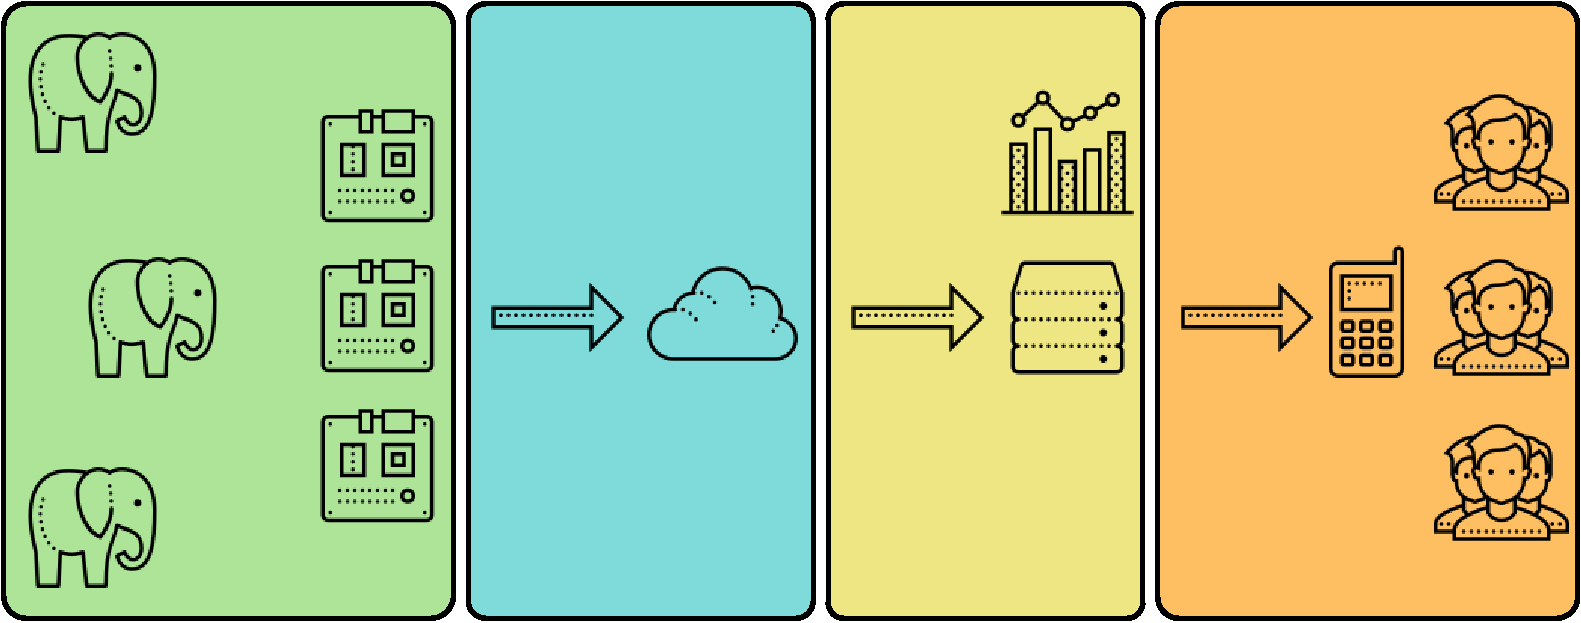
\includegraphics[width=1.0\linewidth]{early_detection_system.pdf} 
        \caption{Diagram of early detection system. Icons source: www.icons8.com}
        \label{early_detection_system}
\end{figure}

An appropriate workflow would be that deployed devices take pictures of their surroundings and send them over a wireless network to the main server for processing.

Although most of the villages in Sonitpur district have access to cell phones and the internet, the connectivity can be unreliable\cite{wildlabs-elephants}. 
Furthermore, devices will be placed quite far from the main server, which makes sending a large amount of data a problem. 
This limits choice of wireless networks to long range, low bandwidth technologies.
It is therefore preferable that elephant detection is done on deployed devices and only results (which can be big few bytes) are sent over some radio network to the main server.
Deployed devices will be placed in forests, fields, with no access to electricity, therefore they need to be battery powered.
Low maintenance of deployed devices is a desirable quality, which means that they should be functional for longer periods without any human interactions.
To achieve that with a limited power source, they should be energy efficient, equipped with solar panels, and a low power radio.
Devices should spend most of their time in sleep mode, conserving energy, only waking up to take a photo, processing it, and sending results to the main server.
As most of the human-elephant conflicts happen during night\cite{wildlabs-elephants}, a thermal camera is needed.

Elephant recognition can be done with the help of a convolutional neural network (CNN) running inference on a microcontroller. 
Making this possible and evaluating the solution is the focus of this master's thesis.


\section{ IRNAS and Arribada Initiative}

The system described above is currently in development at IRNAS in collaboration with Arribada Initiative.
Slovenia based Institute IRNAS offers a complete development service, starting with an idea on paper and ending with a finished product. 
Its previous projects cover a wide range of different fields, from free space optical systems, bio-printing, to Internet of things (IoT) solutions that cover various industrial and nature conservative use cases.
Arribada Initiative is a London based team, that uses open source solutions for purposes of nature conservation.
As the winner of WWF and WILDLABS Human Wildlife Conflict Tech Challenge\cite{wildlabs-winners}, Arribada received funding to develop an early detection system.
They spent some time in Assam, India, where they tested proof-of-concept design\cite{arribada-assam}.
They decided on devices with thermal cameras, as human-elephant conflicts often happen during the night.
The sensor of choice was FLIR Lepton 2.5 and/or 3.5.
They also created a large dataset of elephants pictures while filming elephants in Whipsnade's zoo in the United Kingdom. 
This dataset will be important for training the neural network and it will be discussed in TODO: ADD CHAPTER NUMBER.
To create a final embedded system with on device machine learning, Arribada chose to work with IRNAS.


\section{ Background}

It is worth describing the field of machine learning and its current position in the world of small, embedded devices before continuing to objectives of this master's thesis.
We will only mention some high-level concepts of machine learning in this section, low-level details specific to neural networks will be described in section TODO: ADD SECTION NUMBER.

\subsection{ Machine learning in general}

According to Arthur Samuel (qtd. in Geron \cite{geron}) machine learning (ML) is a field of study that gives computers the ability to learn without being explicitly programmed.
This ability to learn is the property of various machine learning algorithms.
We will be using "machine learning" and "learning" terms interchangeably. 
In order to learn, these learning algorithms need to be trained on a collection of examples of some phenomenon\cite{burkovml}. 
These collections are called \textbf{datasets} and can be generated artificially or collected in nature.

An example of a ML application is a system that can predict a type of animal movement from an accelerometer sensor.
To train its learning algorithm, also known as a \textbf{model}, we need to expose it to a dataset which would contain accelerometer measurements of different types of movement, such a walking, running, jumping and standing still.
Input to the system could be either raw measurements from all three axis or components extracted from raw measurements such as frequency or amplitude. 
These inputs are also known as \textbf{features}, they are values that describe the phenomenon being observed\cite{burkovml}. 
The output of the system would be a predicted type of movement.
Although we would label each example of measurement data what type of movement it represents, we would not directly define the relationship between the two.
Instead, we would let the model figure out connection by itself, through the process of training.
The trained model should be general enough so it can correctly predict the type of movement on unseen accelerometer data.

There exists a large variety of different learning algorithms. 
We can broadly categorize them in several ways, one of them depends on how much supervision learning algorithms need in the training process. 
Algorithms like K-nearest neighbours, linear and logistic regression, support vector machines fall into the category of supervised learning algorithms.
Training data that is fed into them includes solutions, also known as \textbf{labels}\cite{geron}.
Described example is an example of a supervised learning problem.

Algorithms like k-Means, Expectation Maximization, Principal Component Analysis fall into the category of unsupervised learning algorithms.
Here training data is unlabeled, algorithms are trying to find similarities in data by itself\cite{geron}.
There exist other categories such as semi-supervised learning which is a combination of previous two and reinforcement learning, where model acts inside environment according to learned policies\cite{geron}.

Neural networks, algorithms inspired by neurons in human brains\cite{geron}\cite{cs231n}, can fall into either of categories. 
They are appropriate for solving complex problems like image classification, speech recognition, and autonomous driving, but they require a large amount of data and computing power to function correctly.
They fall into field of deep learning, which is a sub-field of machine learning.

Today ML algorithms are present in many software products that we often use. 
They can be found in email spam detection, recommendation algorithms on Facebook and YouTube, speech recognition on smartphones, and virtual personal assistants. 

Training of deep learning algorithms is computationally demanding and is usually done on powerful servers or computers with dedicated graphic processing units to speed up training time.
After a model has been trained, they can feed it data and get prediction in return. 
This process is also known as \textbf{inference}.
The inference is computationally less intensive compared to the training process, so with properly optimized models, we can run inference on personal computers, smartphones, tablets, and even directly in internet browsers.


\subsection{ Machine learning on embedded devices}

Machine learning on embedded devices is an emerging field, which nicely coincides with the Internet of things.
Resources about it are limited, especially when compared to the wast number of resources connected with machine learning on computers or servers.
Most of the information about it can be found in form of scientific papers, blog posts and machine learning framework documentation\cite{hello_edge}\cite{tflite_risc-v}\cite{pete_tiny}.

Running learning algorithms directly on smart devices comes with many benefits.
One of them is reduced power consumption.
In most IoT applications devices send raw sensor data over a wireless network to the server, which processes it either for visualization or for making informed decisions about the system as a whole. 
Wireless communication is one of the more power hungry operations that embedded devices can do, while computation is one of more energy efficient\cite{pete_tiny}.
For example, a Bluetooth communication might use up to 100 milliwatts, while MobileNetV2 image classification network running 1 inference per second would use up to 110 microwatts\cite{pete_tiny}
As deployed devices are usually battery powered, it is important to keep any wireless communication to a minimum, minimizing the amount of data that we send is paramount.
Instead of sending everything we capture, is much more efficient to process raw data on the devices and only send results.

Another benefit of using ML on embedded devices is decreased time between event and action.
If the devices can extract high-level information from raw data, they can act on it immediately, instead of sending it to the cloud and waiting for a response. 
Getting a result now takes milliseconds, instead of seconds.

Such benefits do come with some drawbacks.
Embedded devices are a more resource constrained environment when compared to personal computers or servers.
Because of limited processing power, it is not feasible to train ML models directly on microcontrollers.
Also is not feasible to do online learning with microcontrollers, meaning that they would learn while being deployed.
Models also need to be small enough to fit on a device. 
Most general purpose microcontrollers only offer several hundred kilobytes of flash, up to 2 megabytes.
For comparison, MobileNet v1 image classification model, optimized for mobile phones, is 16.9 MB in size\cite{daniel_edgeimpulse}.
To make it fit on a microcontroller and still have space for our application, we would have to greatly simplify it.

Usual workflow, while developing machine learning models for microcontrollers, is to train a model on training data on some powerful computer or server. 
When we are satisfied with the accuracy of the model we then quantize it (more about quantization in chapter TODO: ADD CHAPTER NUMBER, SHOULD THIS BE A FOOTNOTE?) and convert it into a format understandable to our microcontroller.

There are several frameworks, proprietary and open-sourced, that can be used to develop ML applications on microcontrollers.
STMicroelectronics created X-CUBE-AI, a tool that converts the pre-trained model created by one of the various Deep Learning frameworks into an optimized library. 
X-CUBE-AI works only with STM32 microcontrollers and is proprietary.
Another framework, TensorFlow Lite, was created as an extension of TensorFlow, an open-source software library used for ML applications.
It provides converter tools and C++ implementations of common ML operations, that can run on any microcontroller.

\section{ Objective}

The objective of this master's thesis is to build a device that will be able to recognize elephants and humans from images captured by a thermal camera and report its results to a remote server.
For that, we will have to train a neural network model capable of classifying elephants and humans from thermal images.
After we implement this model on a microcontroller, we will design a printed circuit board (PCB) that will connect microcontroller with various sensors and peripherals.
The device will be battery powered, so minimizing power consumption will necessary.
The device will use LoRa radio to communicate with a remote server.

\section{ Master's thesis outline}
This chapter provided an overview of motivation and companies involved, some background knowledge about machine learning, and the objectives of this thesis.
Chapter 2 will provide a theoretical description of system building blocks. Thermal camera FLIR Lepton, LoRa, neural networks, TensorFlow Lite, and others will be discussed there.
Chapter 3 will revolve around the design and implementation of the device, from hardware and software perspectives.
In chapter 4 we will test our device and present results.
Chapter 5 will present our findings, describe the limitations of our project, and suggest paths for further research.

